\begin{scanpage}{0075}{58}
\begin{minipage}[t]{.43\linewidth}\vspace{0pt}\centering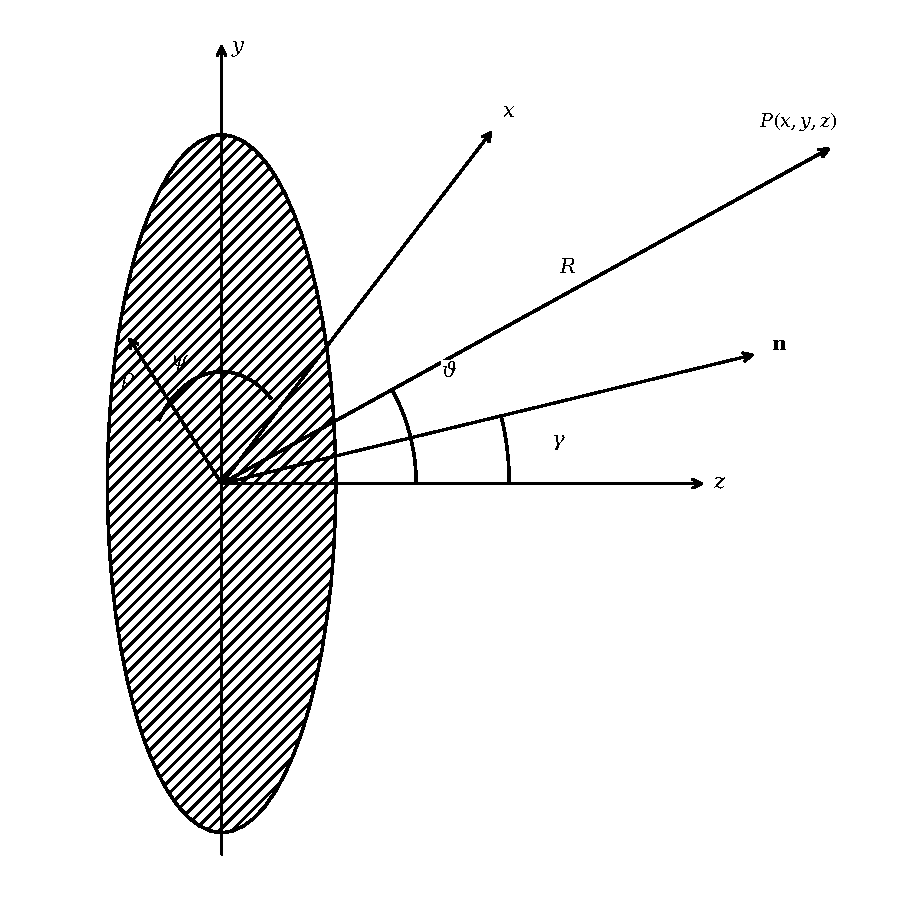
\includegraphics[width=.8\linewidth]{images/recreated/a-0075-fig22.pdf}\par Figure 22. The oblique incidence of a plane wave on a disk. $\mathbf n$ is the normal to the incident wave front.\end{minipage}\hfill\begin{minipage}[t]{.53\linewidth}\vspace{0pt}
\[\psi_1=\delta,\quad\psi_2=\pi+\delta\tag{11.04}\]
are the stationary phase points and the quantity $\delta$ is determined by the equalities
\[\sin\delta=\frac\mu{\sqrt{\lambda^2+\mu^2}},\quad\cos\delta=\frac\lambda{\sqrt{\lambda^2+\mu^2}}.\tag{11.05}\]
From Equation (11.03) it follows that with $R\gg ka^2$ and $ka\sqrt{\lambda^2+\mu^2}\gg1$ the main contribution to the fringing field is given
\end{minipage}
by the luminous region adjacent to the line $\psi=\psi_1$, $\psi=\psi_2$. Thus, the stationary phase points $\psi_1$, $\psi_2$ physically correspond to the luminous line on the disk surface.

In order to calculate the vector potential (11.03), it is necessary for us to first express the nonuniform part of the current on the half-plane in terms of its field in the far zone. For this purpose, let us introduce the auxiliary coordinate systems $x_1,y_1$ and $x_2,y_2$ (see Figure 23), and let us take the following designations:

$\alpha_1,\beta_1$ $(\alpha_2,\beta_2)$ are the angles between the normal to the incident wave front and the coordinate axes $x_1,y_1$ $(x_2,y_2)$;

$\phi_1^0$ $(\phi_1^0=-\phi_2^0)$ is the angle between the $z$ axis and the projection of the indicated normal on the plane $x_1=0$;

$\phi_1$ $(\phi_1=-\phi_2)$ is the angle between the $z$ axis and the direction from the coordinate origin to the point $p(y_1,z)$ which lies in the plane $x_1=0$ and is the projection of the observation point $P(x,y,z)$;

$r_1$ is the distance from the origin to the point $p(y_1,z)$.

The quantities introduced here are determined by the equations:
\end{scanpage}
